\documentclass[../../Installationguide_Unity_Pupil]{subfiles}
% Hier müssen keine Packages geladen werden, es werden automatisch die von masterdoc geladen,
% sowie die Konfigurationen.
% Bei includegraphics nur Bildname (Bsp: Bild.png) eingeben, da er in den angegebenen Pfade die Bilder sucht
\graphicspath{{img/}{../../img/}}

\begin{document}

\chapter{Installation of Unity}
Estimated time for installation: 1 hour 30 minutes

\section{Unity}
Unity is a 3D engine for multi-platform game development. It's a tool to create 3D and 2D games with a focus on easy entry area for developers. We use Unity to build Virtual Reality and Augmented Reality applications.

\begin{enumerate}
	\item Download \href{https://unity3d.com/en/get-unity/download/archive}{Unity version 5.5.1f} and install it. 
	\item In the next step create a new project. Click on the ``NEW'' button (Fig. \ref{fig:pic3}) and fill in the details of the project (Fig. \ref{fig:pic4}). The project name and its location are up to your personal preference.
	\begin{figure}[htb]
		\centering
		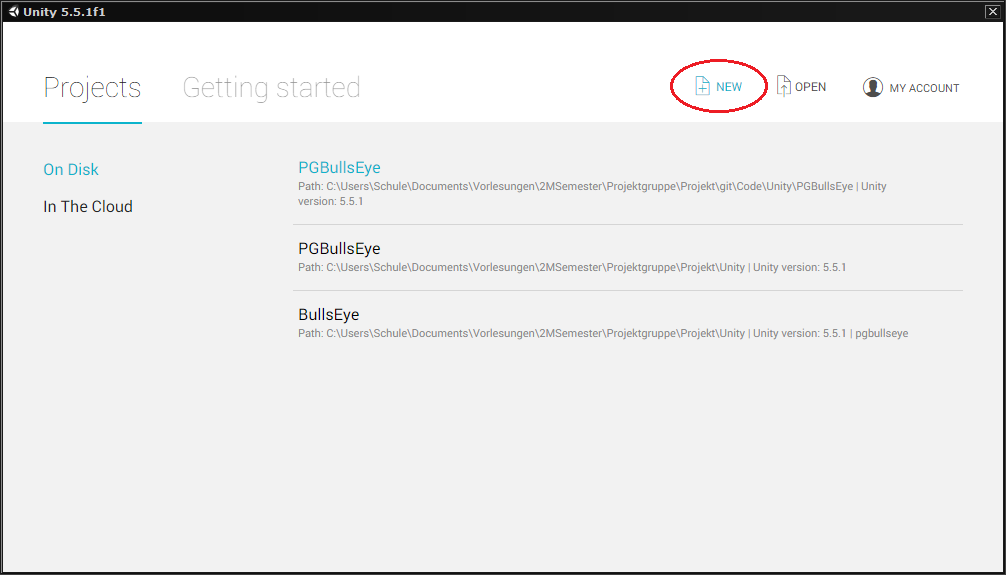
\includegraphics[width=0.95\linewidth]{img/pic3}
		\caption{Launch menu of Unity: The red circle marks the button for creating a new project.}
		\label{fig:pic3}
	\end{figure}
\begin{figure}[htb]
	\centering
	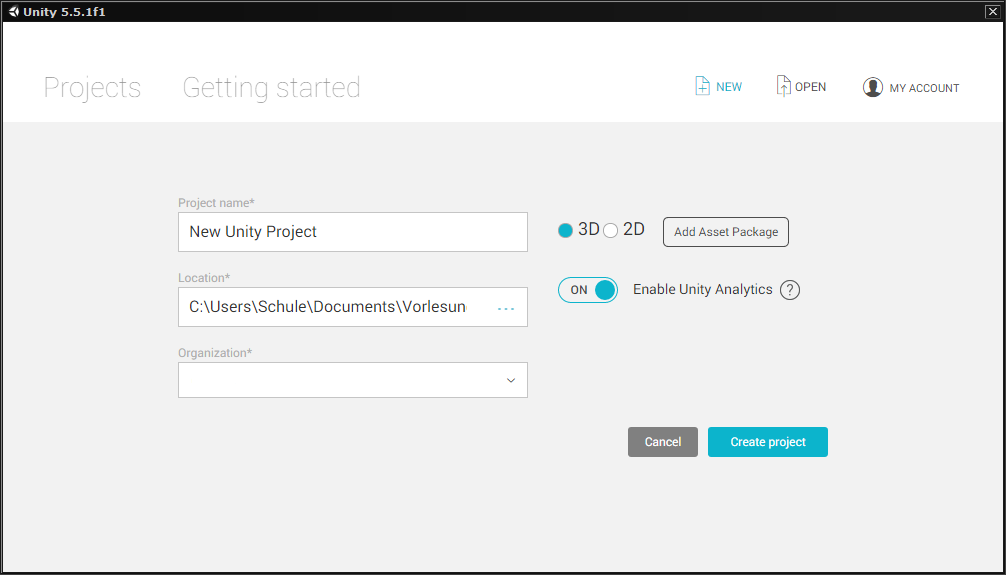
\includegraphics[width=0.95\linewidth]{img/pic4}
	\caption{}
	\label{fig:pic4}
\end{figure}
\item Import the provided unitypackage ``PGBullsEye'' into the newly created project. To do this choose Assets $\rightarrow$ Import Packages $\rightarrow$ Custom Packages $\rightarrow$ PGBullsEye (Fig. \ref{fig:pic5}). This import might take up to several minutes.
	\begin{figure}[htb]
		\centering
		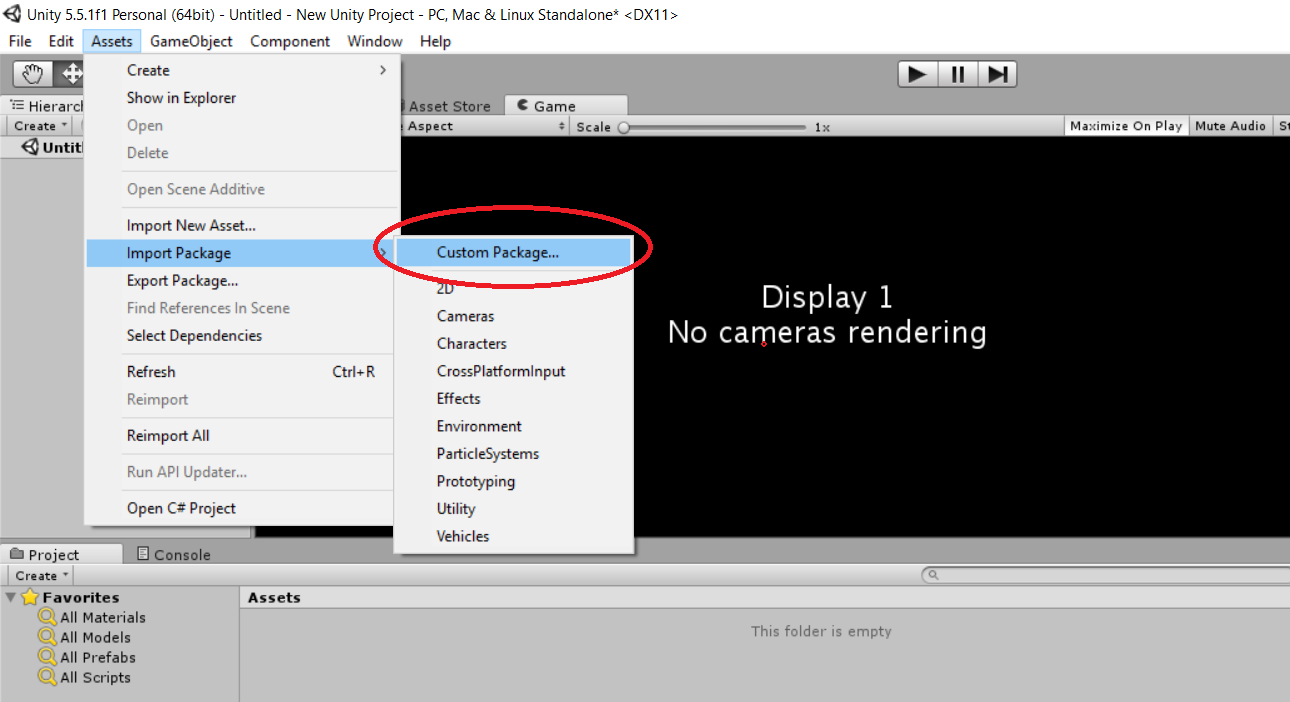
\includegraphics[width=0.95\linewidth]{img/pic5}
		\caption{Import the Unity package ``PGBullsEye''}
		\label{fig:pic5}
	\end{figure}	
\end{enumerate}
\clearpage

\section{Android SDK setup}
The Android Software Development Kit (SDK) is required to build applications for Android smartphones. Unfortunatly you can't download the Android SDK seperatly, it can be only downloaded along with the Integrated Development Environment (IDE) Android Studio.

\begin{enumerate}
\item First download \href{https://developer.android.com/studio/index.html}{Android Studio}, install and start it.
Click  on Configure $\rightarrow$ SDK Manager to open the SDK Manager (see figure \ref{fig:1}).
\begin{figure}[htb]
	\centering
	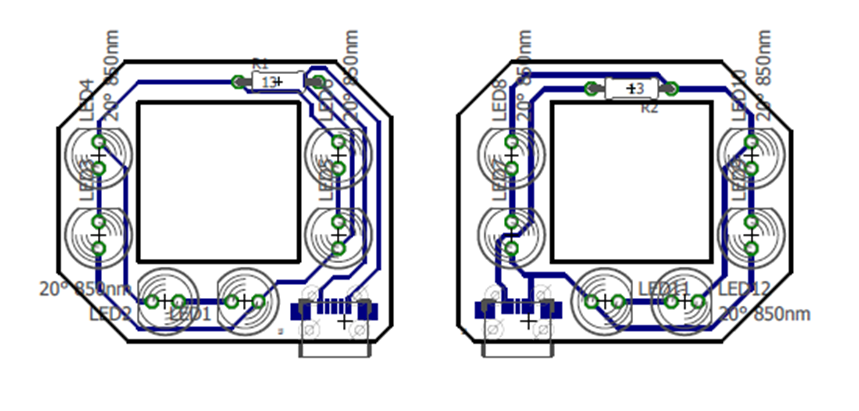
\includegraphics[width=0.75\linewidth]{img/1}
	\caption{Launch menu of Android Studio}
	\label{fig:1}
\end{figure}
\item Under Android SDK $\rightarrow$ SDK Platforms select  Android 7.0 Api 24  (Figure \ref{fig:3}). This Android version is required to build the android application with Unity 5.5.1f.
\begin{figure}[htb]
	\centering
	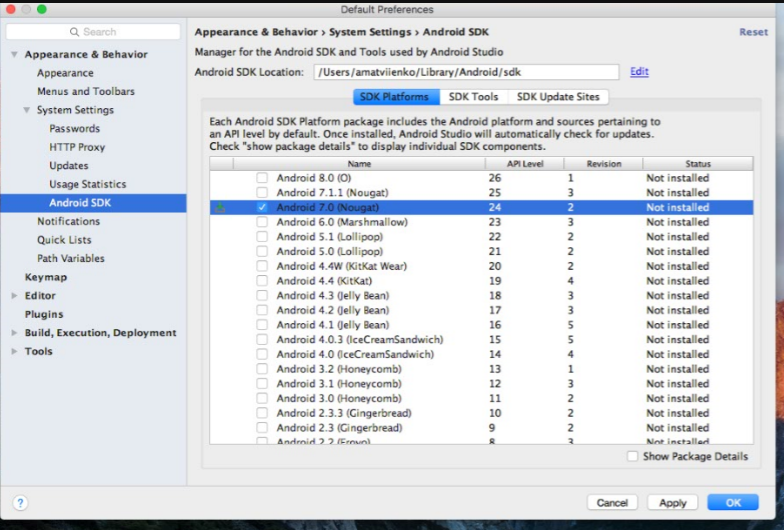
\includegraphics[width=0.95\linewidth]{img/3}
	\caption{Selection of Android 7.0 in the SDK Manager}
	\label{fig:3}
\end{figure}
\item For SDK Tools select the three elements (Figure \ref{fig:4}) and click on apply. The specified items are downloaded. This may take some time. Note the path of the AndroidSDKLocation. 
\begin{figure}[htb]
	\centering
	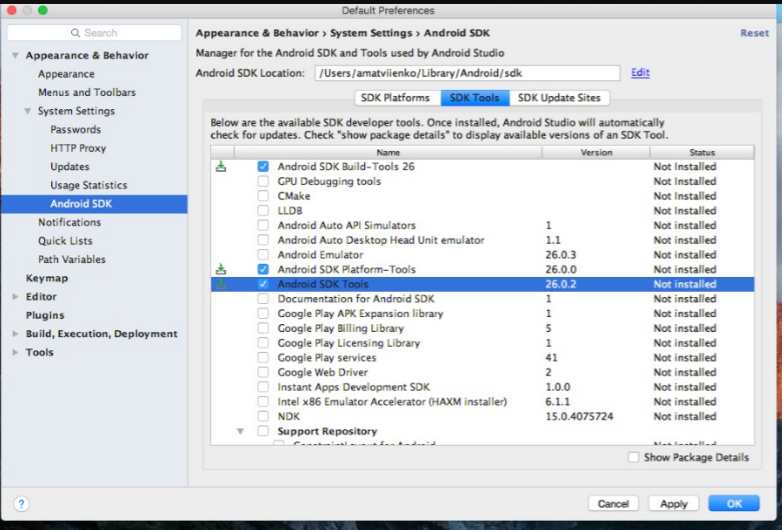
\includegraphics[width=0.95\linewidth]{img/4}
	\caption{Selection of Android SDK Tools, Build-Tools and Platform-Tools in the SDK Manager}
	\label{fig:4}
\end{figure}
\item Open unity as described above. Go to File $\rightarrow$ Build Settings select Android as a platform and click Switch Platform. 
\item Go to Unity $\rightarrow$ Preference $\rightarrow$ External Tools and enter the previously noted AndroidSDKLocation (Note that this is JDK8).
\item Download and unzip the file \href{https://drive.google.com/open?id=0Bwi9ngZcxOHjUlhQUmdRQjRuX2M}{tools\_r25.2.5} and overwrite the path from the old SDK version with the unzip file.
\end{enumerate}
The next step is optional and shows how you could get your android device recognized by your system\\
The following steps will be done on the corresponding smartphone device:\\
To enable USB debugging, you need to enable Developer options. To do this, find the build number in your device’s Settings menu. The location of the build number varies between devices. The stock Android setting can be found by navigating to Settings $\rightarrow$ About phone $\rightarrow$ Build number. For different devices and Android versions, refer to your hardware manufacturer (see fig. \ref{fig:pic1}).

\begin{figure}[htb]
	\centering
	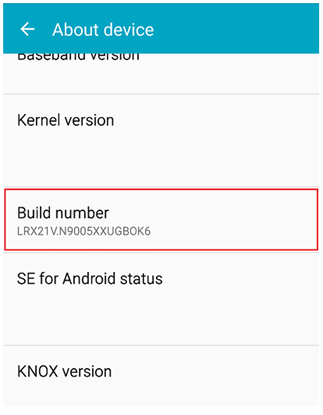
\includegraphics[width=0.5\linewidth]{img/pic1}
	\caption{Tipping on the build number in the phone settings}
	\label{fig:pic1}
\end{figure}

Note: On operating systems older than Android 4.2 (Jelly Bean), the Developer options aren’t hidden. Go to Settings $\rightarrow$ Developer options, then enable USB debugging.
After you have navigated to the build number using the instructions above, tap on the build number seven times. A pop-up notification saying “You are now X steps away from being a developer” appears, with ``X'' being a number that counts down with every additional tap. On the seventh tap, Developer options are unlocked. Go to Settings $\rightarrow$ Developer options, and check the USB debugging checkbox to enable debug mode when the device is connected to a computer via USB (see fig. \ref{fig:pic2}).

\begin{figure}[htb]
	\centering
	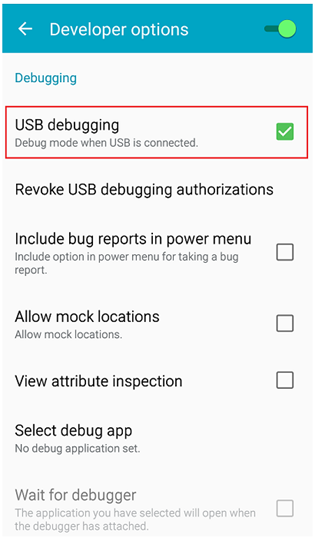
\includegraphics[width=0.5\linewidth]{img/pic2}
	\caption{Enable USB debugging in the developer options}
	\label{fig:pic2}
\end{figure}
\end{document}